% Provenance (never printed): see sources/outline_sources.md (Year 1: internal
% structure of the Earth from seismology; reference model; density, gravity and
% pressure inside the Earth; mantle mineralogy; lithosphere and asthenosphere).
% Curves from figdata/bachelor-1/prem_profiles.py (shared dataset data:prem) and
% figdata/bachelor-1/refraction.py (generic two-layer crust); exercise and problem
% values in the Book 3 scratch calculator calc/ch09.py.
\chapter{La Tierra estratificada}\label{ch:b1:layered-earth}

El 8 de octubre de 1909 un terremoto sacudió el valle del Kupa, al sureste de Zagreb.
% ledger: skoko:mohorovicic
Andrija Mohorovičić, que dirigía el observatorio de la zona, reunió los sismogramas registrados en toda Europa
y notó algo extraño: hasta unos pocos cientos de kilómetros del epicentro, la primera sacudida llegaba de una
manera; más lejos, tomaba el relevo otro tipo de primera llegada, como si parte de la energía hubiera encontrado
un camino más rápido a profundidad. Lo explicó mediante una frontera a unos cincuenta kilómetros de profundidad,
por debajo de la cual las ondas viajan más deprisa: la base de la \omterm{def:b1:layered-earth:layers}{corteza}. Un siglo de registros como aquellos,
millones de ellos, ha convertido aquella primera frontera en un modelo de referencia de toda la Tierra, capa a
capa, con sus velocidades, su densidad, su gravedad y su presión hasta el centro. Este capítulo muestra cómo se
halla una frontera a partir de los tiempos de viaje, qué dice el modelo de referencia, cómo se traza un perfil de
densidad a partir de las velocidades sísmicas solamente y se comprueba con la masa y el momento de inercia de la
Tierra, qué \omterm{def:b1:rock-forming-minerals:mineral}{minerales} forman el \omterm{def:b1:layered-earth:layers}{manto} a cada profundidad, de qué está hecho el núcleo y dónde termina la cáscara
rígida del planeta.

\begin{recall}
Una onda P es una onda de compresión, y una onda S una onda de cizalla; las ondas S no atraviesan los líquidos, y las
zonas de sombra de las ondas P y S del núcleo dan el radio del \omterm{def:b1:layered-earth:layers}{núcleo externo} líquido (libro 2, año 11). Las ondas se
refractan en una frontera según la ley de Snell, $\sin i_1/v_1 = \sin i_2/v_2$ (física). En un fluido en reposo la
presión crece con la profundidad como $\mathrm dP = \rho g\,\mathrm dz$ (física, primer año universitario). La \omterm{def:b1:layered-earth:layers}{corteza},
el \omterm{def:b1:layered-earth:layers}{manto} y el núcleo se presentaron en el libro 1 (año 6).
\end{recall}

\section{Ondas sísmicas en una Tierra estratificada}

Las velocidades de las ondas sísmicas dependen de los módulos elásticos de la roca y de su densidad. Los libros de física
las deducen de las ecuaciones de la elasticidad de medios continuos; aquí se toman como conocidas.

\begin{proposition}[Velocidades sísmicas]\label{prop:b1:layered-earth:speeds}
En un sólido elástico isótropo de densidad $\rho$, módulo de compresión $K$ y módulo de cizalla $\mu$, las ondas P y S
viajan a
\[
  v_P = \sqrt{\frac{K + \tfrac43\mu}{\rho}}, \qquad v_S = \sqrt{\frac{\mu}{\rho}}.
\]
En un líquido $\mu = 0$: $v_S = 0$ y no se propaga ninguna onda S.
\end{proposition}
\admitted

Como $K$ y $\mu$ son positivos, $v_P > v_S$ siempre: en la \omterm{def:b1:layered-earth:layers}{corteza} y el \omterm{def:b1:layered-earth:layers}{manto} del PREM, $v_P$ es unas $1.8$ a $1.9$ veces
$v_S$, y las ondas P llegan primero. Ambas velocidades crecen en general con la profundidad, porque la presión rigidiza la
roca más de lo que la comprime, de modo que los rayos se curvan de nuevo hacia la superficie; y en algunas profundidades
dan un salto.

\begin{definition}[Discontinuidad sísmica, Moho, fronteras núcleo--manto y del núcleo interno]
\label{def:b1:layered-earth:discontinuity}
Una \emph{discontinuidad sísmica}\index{discontinuidad sísmica} es una superficie en el interior de la Tierra a través de
la cual las velocidades sísmicas, la densidad o ambas cambian bruscamente, en un espesor pequeño comparado con una longitud
de onda sísmica. La \emph{discontinuidad de Mohorovičić}\index{discontinuidad de Mohorovičić} (o \emph{Moho}\index{Moho})
es la base de la \omterm{def:b1:layered-earth:layers}{corteza}, donde $v_P$ salta hasta unos \qty{8}{km.s^{-1}}. La \emph{frontera núcleo--manto}\index{frontera núcleo--manto} es la superficie entre el \omterm{def:b1:layered-earth:layers}{manto} silicatado sólido y el \omterm{def:b1:layered-earth:layers}{núcleo externo} líquido; la \emph{frontera del núcleo
interno}\index{frontera del núcleo interno} es la superficie entre el \omterm{def:b1:layered-earth:layers}{núcleo externo} líquido y el \omterm{def:b1:layered-earth:layers}{núcleo interno} sólido.
\end{definition}

\subsection{Refracción en una frontera entre capas}

Tomemos una capa de espesor $h$ y velocidad $v_1$, la \omterm{def:b1:layered-earth:layers}{corteza}, sobre un semiespacio de velocidad $v_2 > v_1$, el \omterm{def:b1:layered-earth:layers}{manto}, y
una fuente en la superficie. Tres ondas llegan a un receptor a la distancia $x$. La onda directa viaja en la capa, a $v_1$.
La onda reflejada rebota en la frontera. Y un rayo que incide sobre la frontera con el ángulo crítico $i_c$, con
$\sin i_c = v_1/v_2$, se refracta a lo largo de ella, viaja en el medio más rápido justo debajo a la velocidad $v_2$ y
devuelve energía hacia arriba, a la capa, con el mismo ángulo $i_c$ a lo largo de todo su recorrido.

\begin{definition}[Onda de cabeza, distancia de cruce]\label{def:b1:layered-earth:head-wave}
Una \emph{onda de cabeza}\index{onda de cabeza} es la onda que viaja a lo largo de una frontera a la velocidad del medio
más rápido situado debajo y sale de ella hacia arriba con el ángulo crítico. La \emph{distancia de cruce}\index{distancia de cruce} es la distancia a la fuente a partir de la cual la onda de cabeza llega antes que la onda directa.
\end{definition}
\begin{theorem}[Tiempos de viaje en una Tierra de dos capas]\label{thm:b1:layered-earth:two-layer}
Sobre una capa de espesor $h$ y velocidad $v_1$ apoyada en un semiespacio de velocidad $v_2 > v_1$, una fuente y un
receptor en la superficie a la distancia $x$ dan
\[
  t_{\text{directa}} = \frac{x}{v_1}, \qquad
  t_{\text{cabeza}} = \frac{x}{v_2} + \frac{2h\cos i_c}{v_1}
  \quad (x \ge 2h\tan i_c), \qquad \sin i_c = \frac{v_1}{v_2},
\]
y la \omterm{def:b1:layered-earth:head-wave}{onda de cabeza} llega primero más allá de la \omterm{def:b1:layered-earth:head-wave}{distancia de cruce}
\[
  x_c = 2h\sqrt{\frac{v_2 + v_1}{v_2 - v_1}}.
\]
\end{theorem}

\begin{proof}
La \omterm{def:b1:layered-earth:head-wave}{onda de cabeza} desciende con el ángulo $i_c$ a través de la capa, por un camino de longitud $h/\cos i_c$, recorre la
frontera a lo largo de la distancia $x - 2h\tan i_c$ y sube por un camino de longitud $h/\cos i_c$. Su tiempo de viaje es
\[
  t_{\text{cabeza}} = \frac{2h}{v_1\cos i_c} + \frac{x - 2h\tan i_c}{v_2}
  = \frac{x}{v_2} + \frac{2h}{v_1\cos i_c}\Bigl(1 - \frac{v_1\sin i_c}{v_2}\Bigr)
  = \frac{x}{v_2} + \frac{2h}{v_1\cos i_c}\,(1 - \sin^2 i_c),
\]
que es $x/v_2 + 2h\cos i_c/v_1$. El camino existe solo si el recorrido horizontal es positivo, $x \ge 2h\tan i_c$. Los dos
tiempos son iguales cuando $x(1/v_1 - 1/v_2) = 2h\cos i_c/v_1$; con $\cos i_c = \sqrt{v_2^2 - v_1^2}/v_2$,
\[
  x\,\frac{v_2 - v_1}{v_1 v_2} = \frac{2h\sqrt{(v_2 - v_1)(v_2 + v_1)}}{v_1 v_2},
\]
que da $x_c$. Más allá de él, la recta de la \omterm{def:b1:layered-earth:head-wave}{onda de cabeza}, de pendiente menor $1/v_2$, queda por debajo de la recta
de la onda directa.
\end{proof}

En un gráfico de tiempo de viaje frente a distancia, las ondas directa y de cabeza son dos rectas. Sus pendientes son las
velocidades inversas $1/v_1$ y $1/v_2$; la recta de la \omterm{def:b1:layered-earth:head-wave}{onda de cabeza}, prolongada hasta $x = 0$, corta el eje de tiempos en el
\emph{tiempo de intersección} $t_i = 2h\cos i_c/v_1$. La onda reflejada,
$t = \sqrt{x^2 + 4h^2}/v_1$, es una hipérbola que toca la recta de la \omterm{def:b1:layered-earth:head-wave}{onda de cabeza} en la distancia crítica $2h\tan i_c$,
donde nace la \omterm{def:b1:layered-earth:head-wave}{onda de cabeza} (\cref{exo:b1:layered-earth:10}).

\begin{omfigure}
\begin{tabular}{@{}c@{}}
\begin{tikzpicture}
\begin{axis}[width=0.86\linewidth, axis equal image, xmin=0, xmax=260, ymin=-62, ymax=8,
  axis x line=top, axis y line=left, axis line style={-}, clip=false,
  ylabel={profundidad (km)}, ytick={-60,-35,0},
  yticklabels={60,35,0}, tick label style={font=\scriptsize}, label style={font=\small}]
\fill[brown!12] (axis cs:0,0) rectangle (axis cs:260,-35);
\fill[orange!18] (axis cs:0,-35) rectangle (axis cs:260,-62);
\draw[black!60] (axis cs:0,-35) -- (axis cs:260,-35);
\addplot[very thick, blue!70!black] table[x=x, y=z, unbounded coords=jump,
  restrict expr to domain={\coordindex}{0:1}] {figdata/out/bachelor-1-refraction-rays.dat};
\addplot[thick, dashed, green!45!black] table[x=x, y=z, unbounded coords=jump,
  restrict expr to domain={\coordindex}{3:5}] {figdata/out/bachelor-1-refraction-rays.dat};
\addplot[very thick, red!75!black] table[x=x, y=z, unbounded coords=jump,
  restrict expr to domain={\coordindex}{7:10}] {figdata/out/bachelor-1-refraction-rays.dat};
\node[font=\scriptsize, anchor=north west] at (axis cs:2,-36) {manto, $v_2 = \qty{8.0}{km.s^{-1}}$};
\node[font=\scriptsize, anchor=center] at (axis cs:125,-17) {corteza, $v_1 = \qty{6.0}{km.s^{-1}}$, $h = \qty{35}{km}$};
\node[font=\scriptsize, red!75!black, anchor=north] at (axis cs:150,-36) {onda de cabeza a lo largo del Moho};
\node[font=\scriptsize, green!45!black, anchor=south] at (axis cs:40,-20) {reflejada};
\node[font=\scriptsize, blue!70!black, anchor=north] at (axis cs:125,-1) {directa};
\fill (axis cs:0,0) circle (2pt);
\end{axis}
\end{tikzpicture}\\[2pt]
{\small (a) trayectorias de los rayos (distancia en km)}\\[6pt]
\begin{tikzpicture}
\begin{axis}[omrecord, width=0.86\linewidth, height=6.0cm, xmin=0, xmax=400, ymin=0, ymax=70,
  xlabel={distancia $x$ (km)}, ylabel={tiempo de viaje $t$ (s)}, tick label style={font=\scriptsize},
  label style={font=\small}, clip=false,
  legend style={font=\scriptsize, at={(0.03,0.97)}, anchor=north west, draw=none, fill=white, fill opacity=0.85}]
\addplot[very thick, blue!70!black] table[x=x, y=t_direct] {figdata/out/bachelor-1-refraction-times.dat};
\addlegendentry{directa, pendiente $1/v_1$}
\addplot[thick, dashed, green!45!black] table[x=x, y=t_reflected] {figdata/out/bachelor-1-refraction-times.dat};
\addlegendentry{reflejada}
\addplot[very thick, red!75!black, unbounded coords=jump] table[x=x, y=t_head] {figdata/out/bachelor-1-refraction-times.dat};
\addlegendentry{onda de cabeza, pendiente $1/v_2$}
\addplot[thin, dotted, red!75!black, domain=0:79.37] {x/8 + 7.717};
\draw[black!60, densely dashed] (axis cs:185.2,0) -- (axis cs:185.2,30.87);
\node[font=\scriptsize, anchor=north west] at (axis cs:187,8) {$x_c = \qty{185}{km}$};
\node[font=\scriptsize, anchor=east, red!75!black] at (axis cs:-3,7.7) {$t_i$};
\end{axis}
\end{tikzpicture}\\[2pt]
{\small (b) tiempos de viaje}
\end{tabular}

\par\smallskip{\small Refracción sobre una \omterm{def:b1:layered-earth:layers}{corteza} de \qty{35}{km} de espesor, a \qty{6.0}{km.s^{-1}}, sobre un \omterm{def:b1:layered-earth:layers}{manto} a
\qty{8.0}{km.s^{-1}} ((a) a escala verdadera). (a) La onda directa recorre la superficie; la onda reflejada dibujada es la que
incide sobre el \omterm{def:b1:layered-earth:discontinuity}{Moho} con el ángulo crítico, \ang{48.6}; la \omterm{def:b1:layered-earth:head-wave}{onda de cabeza} recorre el \omterm{def:b1:layered-earth:discontinuity}{Moho} y vuelve con ese ángulo. (b)
Tiempos de llegada: la \omterm{def:b1:layered-earth:head-wave}{onda de cabeza} aparece a la distancia crítica, \qty{79}{km}, tangente a la reflexión, y adelanta a la
onda directa a la \omterm{def:b1:layered-earth:head-wave}{distancia de cruce}, \qty{185}{km}. La prolongación punteada da el tiempo de intersección
$t_i = \qty{7.7}{s}$.}
\end{omfigure}

\begin{method}[La profundidad de una frontera a partir de un perfil de refracción]\label{met:b1:layered-earth:moho}
\begin{enumerate}
  \item Represéntense los tiempos de primera llegada frente a la distancia, y ajústese una recta a las llegadas cercanas a la
        fuente y otra a las lejanas.
  \item Las inversas de las pendientes dan $v_1$ y $v_2$; después $\sin i_c = v_1/v_2$.
  \item Léase el tiempo de intersección $t_i$ de la recta lejana en $x = 0$, y calcúlese $h = t_i v_1/(2\cos i_c)$; compruébese con
        la \omterm{def:b1:layered-earth:head-wave}{distancia de cruce}, $h = \tfrac12 x_c\sqrt{(v_2 - v_1)/(v_2 + v_1)}$.
  \item Una frontera solo se encuentra si $v_2 > v_1$: una capa más lenta debajo de otra más rápida no produce \omterm{def:b1:layered-earth:head-wave}{onda de cabeza} y
        permanece oculta.
\end{enumerate}
\end{method}

Las dos clases de primera llegada de Mohorovičić fueron exactamente estas dos rectas: la onda directa en la \omterm{def:b1:layered-earth:layers}{corteza} cerca de la
fuente, y la \omterm{def:b1:layered-earth:head-wave}{onda de cabeza} a lo largo de la parte superior del \omterm{def:b1:layered-earth:layers}{manto} más lejos. Su figura para el espesor de la \omterm{def:b1:layered-earth:layers}{corteza} en esa
región, \qty{54}{km}, se ha confirmado en su orden de magnitud, pero la profundidad del \omterm{def:b1:layered-earth:discontinuity}{Moho} varía de un lugar a otro. Bajo los
océanos la \omterm{def:b1:layered-earth:layers}{corteza} tiene solo unos \qty{5}{km} de espesor; bajo los continentes, de media unos \qty{30}{km}, y es mucho más gruesa
bajo las grandes cordilleras. Para su modelo de referencia, el PREM situó el \omterm{def:b1:layered-earth:discontinuity}{Moho} a \qty{11}{km} bajo el nivel del mar bajo los
océanos y a \qty{35}{km} bajo los continentes.
% ledger: skoko:mohorovicic, usgs:crust-thickness, prem:moho-average

\begin{history}[Andrija Mohorovičić]
\begin{minipage}[t]{0.76\linewidth}\vspace{0pt}
% ledger: skoko:mohorovicic
Andrija Mohorovičić (1857--1936) llegó a la sismología desde la meteorología: maestro, y después, de 1891 a 1921, director del
observatorio meteorológico de Zagreb; publicó su último estudio meteorológico en 1901. En los sismogramas del terremoto del valle
del Kupa, del 8 de octubre de 1909, halló dos parejas distintas de fases P y S: cerca de la fuente llegaba una clase de primera
sacudida, y más lejos otra, que había viajado más deprisa a profundidad. Su lectura de estas dos llegadas como una onda directa
y una onda refractada bajo una frontera dio la frontera que hoy lleva su nombre, y la primera medida del espesor de la \omterm{def:b1:layered-earth:layers}{corteza}.
\end{minipage}\hfill
\begin{minipage}[t]{0.2\linewidth}\vspace{0pt}
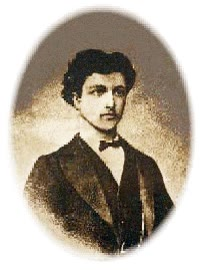
\includegraphics[width=\linewidth]{images/book3/b1-mohorovicic.jpg}

{\scriptsize Andrija Mohorovičić. Dominio público.}
\end{minipage}
\end{history}

\section{Un modelo de Tierra de referencia}

El mismo razonamiento, aplicado a millones de tiempos de viaje a todas las distancias y a los periodos de las oscilaciones
libres de la Tierra (todo el planeta suena como una campana tras un gran terremoto), da las velocidades a cada profundidad.

\begin{definition}[Modelo de Tierra de referencia]\label{def:b1:layered-earth:reference-model}
Un \emph{modelo de Tierra de referencia}\index{modelo de Tierra de referencia} es una Tierra con simetría esférica, dada
como las velocidades sísmicas $v_P(r)$, $v_S(r)$, la densidad $\rho(r)$ y, en los modelos más completos, la atenuación en
función del radio $r$ solamente, que ajusta los tiempos de viaje observados, los periodos de oscilación libre, la masa de la
Tierra y su momento de inercia. El más usado es el PREM, el Modelo Preliminar de Tierra de Referencia (1981).
\end{definition}

El PREM se ajustó al radio \qty{6371}{km}, a la masa \qty{5.974e24}{kg} y al \omterm{def:b1:comparative-planetology:moi}{factor de momento de inercia} $0.3308$ de la
Tierra. Divide el planeta en unas pocas regiones unidas por discontinuidades, y sus perfiles (figura siguiente) muestran de
inmediato las capas principales.

\begin{definition}[Corteza, manto, núcleo externo, núcleo interno]\label{def:b1:layered-earth:layers}
La \emph{corteza}\index{corteza} es la capa silicatada exterior, por encima del \omterm{def:b1:layered-earth:discontinuity}{Moho}. El
\emph{manto}\index{manto} es la cáscara silicatada sólida entre el \omterm{def:b1:layered-earth:discontinuity}{Moho} y la \omterm{def:b1:layered-earth:discontinuity}{frontera núcleo--manto}, a una profundidad de
unos \qty{2891}{km}. El \emph{núcleo externo}\index{núcleo externo} es la cáscara metálica líquida entre la \omterm{def:b1:layered-earth:discontinuity}{frontera
núcleo--manto} y la \omterm{def:b1:layered-earth:discontinuity}{frontera del núcleo interno}, a unos \qty{5150}{km} de profundidad. El \emph{núcleo interno}\index{núcleo interno} es la esfera metálica sólida situada debajo, de radio unos \qty{1220}{km}.
\end{definition}

\begin{omfigure}
\begin{tikzpicture}
\begin{axis}[omrecord, omdepth, width=0.62\linewidth, height=5.4cm, xmin=0, xmax=14, ymin=0, ymax=6371,
  xlabel={velocidad (\unit{km.s^{-1}}) o densidad (\unit{g.cm^{-3}})}, ylabel={profundidad (km)},
  ytick={0,1000,...,6000}, tick label style={font=\scriptsize}, label style={font=\small},
  clip=false, legend style={font=\scriptsize, at={(0.02,0.80)}, anchor=north west, draw=none, fill=white}]
\addplot[very thick, blue!70!black] table[x=vp, y=depth] {figdata/out/bachelor-1-prem_profiles-profiles.dat};
\addlegendentry{$v_P$}
\addplot[very thick, red!75!black] table[x=vs, y=depth] {figdata/out/bachelor-1-prem_profiles-profiles.dat};
\addlegendentry{$v_S$}
\addplot[very thick, black!70, densely dashed] table[x=rho, y=depth] {figdata/out/bachelor-1-prem_profiles-profiles.dat};
\addlegendentry{$\rho$}
\draw[black!35] (axis cs:0,670) -- (axis cs:14,670) node[right, font=\scriptsize, black] {670 km};
\draw[black!35] (axis cs:0,2891) -- (axis cs:14,2891) node[right, font=\scriptsize, black] {frontera núcleo--manto};
\draw[black!35] (axis cs:0,5149.5) -- (axis cs:14,5149.5) node[right, font=\scriptsize, black] {frontera del núcleo interno};
\node[font=\scriptsize, anchor=west] at (axis cs:14,1700) {manto};
\node[font=\scriptsize, anchor=west] at (axis cs:14,4000) {núcleo externo (líquido)};
\node[font=\scriptsize, anchor=west] at (axis cs:14,5800) {núcleo interno (sólido)};
\end{axis}
\end{tikzpicture}

\par\smallskip{\small PREM: las velocidades de las ondas P y S y la densidad frente a la profundidad. La velocidad S cae a
cero en el \omterm{def:b1:layered-earth:layers}{núcleo externo} líquido y reaparece, pequeña, en el \omterm{def:b1:layered-earth:layers}{núcleo interno} sólido; en la \omterm{def:b1:layered-earth:discontinuity}{frontera núcleo--manto} la densidad
casi se duplica mientras $v_P$ baja de 13.7 a \qty{8.1}{km.s^{-1}}; los saltos cerca de \qty{400}{km} y \qty{670}{km} acotan la
zona de transición.}
\end{omfigure}

\begin{table}[htbp]
\centering
\footnotesize
\setlength{\tabcolsep}{3pt}
\begin{tabular}{>{\raggedright\arraybackslash}p{0.2\linewidth}rr>{\raggedright\arraybackslash}p{0.47\linewidth}}
\hline
frontera en PREM & profundidad (km) & radio (km) & qué cambia \\
\hline
\omterm{def:b1:layered-earth:discontinuity}{Moho} & 24.4 & 6346.6 & \omterm{def:b1:layered-earth:layers}{corteza} encima, peridotita debajo; $v_P$ de 6.8 a 8.1 \\
discontinuidad de 220 km & 220 & 6151 & base de la \omterm{def:b1:layered-earth:lithosphere}{zona de baja velocidad} en PREM \\
discontinuidad de 400 km & 400 & 5971 & \omterm{def:b1:rock-forming-minerals:groups}{olivino} a wadsleyita (\qty{410}{km} en la mayoría de los estudios) \\
discontinuidad de 670 km & 670 & 5701 & ringwoodita a bridgmanita y ferropericlasa (\qty{660}{km} en la mayoría de los estudios) \\
\omterm{def:b1:layered-earth:discontinuity}{frontera núcleo--manto} & 2891 & 3480 & silicato a hierro líquido; $v_S$ de 7.3 a 0; $\rho$ de 5.57 a 9.90 \\
\omterm{def:b1:layered-earth:discontinuity}{frontera del núcleo interno} & 5149.5 & 1221.5 & hierro líquido a sólido; $v_S$ de 0 a 3.5; $\rho$ de 12.17 a 12.76 \\
\hline
\end{tabular}
\caption{Las principales discontinuidades de PREM (velocidades en \unit{km.s^{-1}}, densidades en
\unit{g.cm^{-3}}). PREM promedia la \omterm{def:b1:layered-earth:layers}{corteza} en \qty{24.4}{km}; las \omterm{def:b1:layered-earth:layers}{cortezas} reales van desde unos
\qty{5}{km} bajo los océanos hasta muchas decenas de kilómetros bajo las cordilleras.}
% ledger: usgs:crust-thickness
\label{tab:b1:layered-earth:prem}
\end{table}

Dos hechos de estos perfiles se observan directamente. La anulación de $v_S$ en el \omterm{def:b1:layered-earth:layers}{núcleo externo} es la sombra de las ondas S
recordada antes: las ondas S no entran en el núcleo más que como ondas P, el núcleo no transmite cizalla, y por tanto es
líquido. Y el \omterm{def:b1:layered-earth:layers}{núcleo interno} transmite ondas S, lentamente: es sólido. Este segundo hecho procede de llegadas P débiles en
lugares donde no debería haber ondas P.

\begin{history}[Inge Lehmann y el núcleo interno]
% ledger: hjortenberg:lehmann
\begin{minipage}[t]{0.76\linewidth}\vspace{0pt}
Inge Lehmann (1888--1993), jefa del departamento de sismología del Instituto Geodésico danés, estudió los registros del
terremoto de Buller de 1929, en Nueva Zelanda, y halló ondas P que llegaban dentro de la zona de sombra, donde el núcleo
debía haberlas desviado. En un artículo de 1936 con el más breve de los títulos, \emph{P$'$}, mostró que podían explicarse si el
núcleo contenía un \omterm{def:b1:layered-earth:layers}{núcleo interno} más pequeño, con una velocidad P mayor, que devuelve parte de la energía hacia la superficie.
Hoy se sabe que su \omterm{def:b1:layered-earth:layers}{núcleo interno} es sólido y que crece lentamente a medida que la Tierra se enfría. También descubrió la
discontinuidad cercana a \qty{220}{km} que lleva su nombre.
\end{minipage}\hfill
\begin{minipage}[t]{0.2\linewidth}\vspace{0pt}
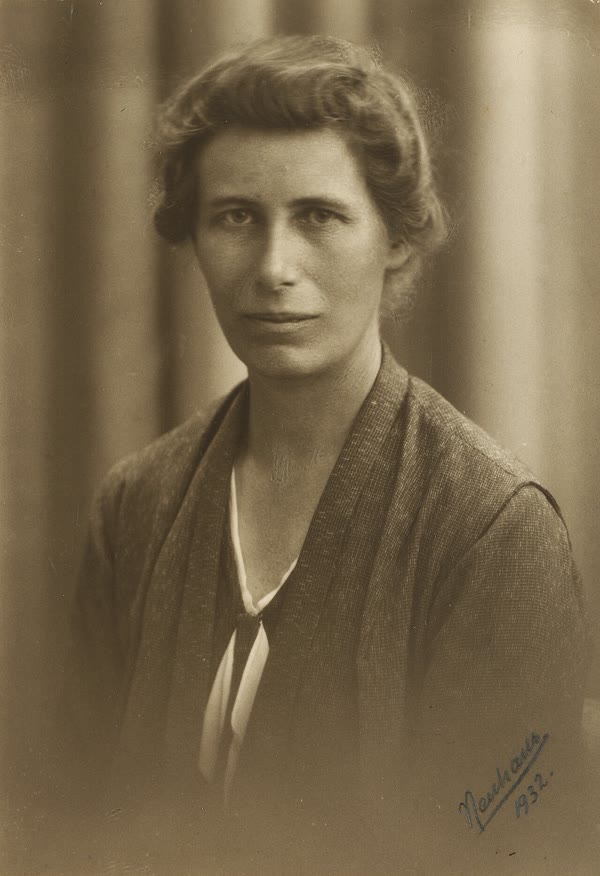
\includegraphics[width=\linewidth]{images/book3/b1-lehmann.jpg}

{\scriptsize Inge Lehmann en 1932, por Even Neuhaus. Dominio público.}
\end{minipage}
\end{history}

\section{Densidad, gravedad y presión a partir de datos sísmicos}

Las velocidades sísmicas dan dos combinaciones de los módulos y de la densidad, no la densidad misma. Una tercera relación
procede de suponer que, dentro de una capa de composición uniforme, la roca se comprime simplemente por el peso de la roca
que tiene encima.

\begin{definition}[Parámetro sísmico]\label{def:b1:layered-earth:seismic-parameter}
El \emph{parámetro sísmico}\index{parámetro sísmico} a una profundidad es
\[
  \Phi = v_P^2 - \tfrac43 v_S^2 = \frac{K}{\rho},
\]
es decir, el módulo de compresión dividido por la densidad, calculado solo a partir de las dos velocidades sísmicas
(\cref{prop:b1:layered-earth:speeds}).
\end{definition}

\begin{theorem}[Ecuación de Adams--Williamson]\label{thm:b1:layered-earth:adams-williamson}
En una región de composición uniforme, en equilibrio hidrostático y comprimida adiabáticamente, la densidad varía con el radio como
\[
  \frac{\mathrm d\rho}{\mathrm dr} = -\frac{\rho(r)\,g(r)}{\Phi(r)},
\]
donde $g(r)$ es la gravedad a la distancia $r$ del centro.
\end{theorem}

\begin{proof}
El equilibrio hidrostático da $\mathrm dP/\mathrm dr = -\rho g$ (el recordatorio, con $\mathrm dz = -\mathrm dr$). El módulo
de compresión se define por $K = \rho\,\mathrm dP/\mathrm d\rho$ para la compresión considerada; para una roca de composición
fija comprimida sin intercambio de calor, es el módulo adiabático que miden las ondas sísmicas, así que
$\mathrm d\rho/\mathrm dP = \rho/K$. Por la regla de la cadena,
\[
  \frac{\mathrm d\rho}{\mathrm dr} = \frac{\mathrm d\rho}{\mathrm dP}\,
  \frac{\mathrm dP}{\mathrm dr} = \frac{\rho}{K}\,(-\rho g) = -\frac{\rho g}{K/\rho}
  = -\frac{\rho g}{\Phi}. \qedhere
\]
\end{proof}

La ecuación falla en una discontinuidad, donde cambian la composición o la estructura cristalina, y allí donde la temperatura se
aparta de la adiabática; pero entre las discontinuidades explica muy bien el aumento observado de la densidad con la profundidad
(panel (c) de la figura siguiente). Partiendo de una densidad en la parte superior de cada región, integrándola hacia abajo, y
ajustando los valores de partida hasta que la masa y el momento de inercia salgan bien, así se construyeron los primeros modelos
de densidad. Los dos números globales son integrales de la densidad.

\begin{proposition}[Masa, gravedad, presión y momento de inercia]
\label{prop:b1:layered-earth:integrals}
Para una Tierra con simetría esférica de radio $R$ y densidad $\rho(r)$, la masa dentro del radio $r$, la gravedad, la presión y el
momento de inercia respecto de un eje que pasa por el centro son
\[
  m(r) = \int_0^r 4\pi s^2\rho(s)\,\mathrm ds, \quad
  g(r) = \frac{G\,m(r)}{r^2}, \quad
  P(r) = \int_r^R \rho(s)\,g(s)\,\mathrm ds, \quad
  I = \frac{8\pi}{3}\int_0^R \rho(r)\,r^4\,\mathrm dr.
\]
\end{proposition}

\begin{proof}
Una cáscara delgada de radio $s$ y espesor $\mathrm ds$ tiene el volumen $4\pi s^2\,\mathrm ds$, de ahí la primera integral. La
gravedad de un cuerpo con simetría esférica fuera de un radio es la de su masa interior, concentrada en el centro, y las cáscaras
exteriores a $r$ tiran sin fuerza neta (el teorema de la cáscara, que se admite de los libros de física); de ahí $g(r)$. Integrando
la ecuación hidrostática desde la superficie, donde $P = 0$, se obtiene $P(r)$. Para el momento de inercia, una cáscara esférica
delgada de masa $\mathrm dm$ y radio $r$ tiene, respecto de los tres ejes $x$, $y$, $z$, momentos cuya suma es
$\int (y^2 + z^2) + (z^2 + x^2) + (x^2 + y^2)\,\mathrm dm = 2r^2\,\mathrm dm$; por simetría los tres son iguales, así que cada uno vale
$\tfrac23 r^2\,\mathrm dm$. Con $\mathrm dm = 4\pi r^2\rho\,\mathrm dr$, sumando las cáscaras se obtiene $I$.
\end{proof}

Para una esfera de densidad uniforme, $I = \tfrac{8\pi}{15}\rho R^5 = 0.4\,MR^2$. El factor $I/MR^2 = 0.3308$ de la Tierra es
menor: su masa se concentra hacia el centro, que es el primer argumento a favor de un núcleo denso. Calculadas solo con la
densidad del PREM, las integrales dan una masa de \qty{5.976e24}{kg} (un \qty{0.06}{\percent} por encima de la medida
\qty{5.972e24}{kg}), un factor $0.3309$, y una presión central de \qty{364}{GPa}, el valor tabulado con el PREM con una precisión
del \qty{0.1}{\percent}.

\begin{omfigure}
\begin{tabular}{@{}c@{\hspace{2mm}}c@{\hspace{2mm}}c@{}}
\begin{tikzpicture}
\begin{axis}[omrecord, omdepth, width=0.35\linewidth, height=7.0cm, xmin=0, xmax=12, ymin=0, ymax=6371,
  xlabel={$g$ (\unit{m.s^{-2}})}, ylabel={profundidad (km)}, ytick={0,1000,...,6000}, xtick={0,4,8,12},
  tick label style={font=\scriptsize}, label style={font=\small}]
\addplot[very thick, blue!70!black] table[x=g, y=depth] {figdata/out/bachelor-1-prem_profiles-functionals.dat};
\draw[black!35] (axis cs:0,2891) -- (axis cs:12,2891);
\draw[black!35] (axis cs:0,5149.5) -- (axis cs:12,5149.5);
\node[font=\scriptsize, anchor=south west] at (axis cs:0.3,2891) {FNM};
\node[font=\scriptsize, anchor=south west] at (axis cs:0.3,5149.5) {FNI};
\end{axis}
\end{tikzpicture}
&
\begin{tikzpicture}
\begin{axis}[omrecord, omdepth, width=0.35\linewidth, height=7.0cm, xmin=0, xmax=400, ymin=0, ymax=6371,
  xlabel={$P$ (GPa)}, ytick={0,1000,...,6000}, yticklabels={}, xtick={0,200,400},
  tick label style={font=\scriptsize}, label style={font=\small}]
\addplot[very thick, red!75!black] table[x=P, y=depth] {figdata/out/bachelor-1-prem_profiles-functionals.dat};
\draw[black!35] (axis cs:0,2891) -- (axis cs:400,2891);
\draw[black!35] (axis cs:0,5149.5) -- (axis cs:400,5149.5);
\node[font=\scriptsize, anchor=south west] at (axis cs:150,2891) {\qty{136}{GPa}};
\node[font=\scriptsize, anchor=south east] at (axis cs:290,5149.5) {\qty{329}{GPa}};
\end{axis}
\end{tikzpicture}
&
\begin{tikzpicture}
\begin{axis}[omrecord, omdepth, width=0.35\linewidth, height=7.0cm, xmin=2, xmax=14, ymin=0, ymax=6371,
  xlabel={$\rho$ (\unit{g.cm^{-3}})}, ytick={0,1000,...,6000}, yticklabels={}, xtick={2,6,10,14},
  tick label style={font=\scriptsize}, label style={font=\small},
  legend style={font=\scriptsize, at={(0.97,0.97)}, anchor=north east, draw=none, fill=white}]
\addplot[very thick, black!55] table[x=rho, y=depth] {figdata/out/bachelor-1-prem_profiles-profiles.dat};
\addlegendentry{PREM}
\addplot[only marks, mark=o, mark size=1.4pt, orange!85!black, each nth point=15, unbounded coords=discard]
  table[x=rho_aw, y=depth] {figdata/out/bachelor-1-prem_profiles-adams.dat};
\addlegendentry{Adams--Williamson}
\end{axis}
\end{tikzpicture}
\\[2pt]
{\small (a) gravedad} & {\small (b) presión} & {\small (c) autocompresión}
\end{tabular}

\par\smallskip{\small En el interior de la Tierra, a partir del PREM. (a) y (b) Gravedad y presión calculadas a partir de la
densidad del PREM con \cref{prop:b1:layered-earth:integrals}: la gravedad se mantiene cerca de \qty{10}{m.s^{-2}} a lo largo del
\omterm{def:b1:layered-earth:layers}{manto}, alcanza un máximo de \qty{10.7}{m.s^{-2}} en la \omterm{def:b1:layered-earth:discontinuity}{frontera núcleo--manto} (FNM) y cae a cero en el centro; la presión llega a
\qty{136}{GPa} en la FNM, a \qty{329}{GPa} en la \omterm{def:b1:layered-earth:discontinuity}{frontera del núcleo interno} (FNI) y a \qty{364}{GPa} en el centro. (c) La ecuación
de Adams--Williamson, integrada hacia abajo desde la densidad del PREM a \qty{771}{km} y en la parte superior del \omterm{def:b1:layered-earth:layers}{núcleo externo} con
las velocidades y la gravedad del PREM (círculos), sigue al PREM con un error inferior al \qty{0.2}{\percent}: allí el aumento de
densidad es la compresión de un material uniforme; los saltos no lo son.}
\end{omfigure}

Que la gravedad crezca al bajar por el \omterm{def:b1:layered-earth:layers}{manto} es una consecuencia directa del núcleo denso: la masa que queda dentro del radio
crece más despacio que $r^2$. A través del \omterm{def:b1:layered-earth:layers}{manto} $g$ apenas cambia, y la presión crece casi linealmente con la profundidad, unos
\qty{4.7}{GPa} por cada cien kilómetros.


\section{El manto: una roca, varias asociaciones minerales}

El \omterm{def:b1:layered-earth:layers}{manto} superior es peridotita, conocida por los fragmentos que traen a la superficie los volcanes y por las láminas de \omterm{def:b1:layered-earth:layers}{manto}
empujadas sobre los continentes: entre la mitad y tres quintos de \omterm{def:b1:rock-forming-minerals:groups}{olivino} en volumen (\qtyrange{49}{62}{\percent} en las
composiciones propuestas), y el resto \omterm{def:b1:rock-forming-minerals:groups}{piroxenos} y un \omterm{def:b1:rock-forming-minerals:mineral}{mineral} alumínico (\omterm{def:b1:rock-forming-minerals:groups}{plagioclasa}, espinela o \omterm{def:b1:rock-forming-minerals:groups}{granate}, según la profundidad).
La presión que crece con la profundidad no cambia esta composición, pero obliga a sus átomos a disponerse en estructuras más
densas: los \omterm{def:b1:rock-forming-minerals:polymorph}{polimorfos} (\cref{ch:b1:rock-forming-minerals}) aparecen uno tras otro.

\begin{definition}[Zona de transición del manto]\label{def:b1:layered-earth:transition-zone}
La \emph{zona de transición del manto}\index{zona de transición del manto} es la parte del \omterm{def:b1:layered-earth:layers}{manto} comprendida entre las
\omterm{def:b1:layered-earth:discontinuity}{discontinuidades sísmicas} cercanas a \qty{410}{km} y \qty{660}{km} de profundidad, en la que el \omterm{def:b1:rock-forming-minerals:groups}{olivino} del \omterm{def:b1:layered-earth:layers}{manto} superior se
sustituye por sus \omterm{def:b1:rock-forming-minerals:polymorph}{polimorfos} más densos, la wadsleyita y luego la ringwoodita. Encima está el \omterm{def:b1:layered-earth:layers}{manto} superior; debajo, el \omterm{def:b1:layered-earth:layers}{manto}
inferior, hasta la \omterm{def:b1:layered-earth:discontinuity}{frontera núcleo--manto}.
\end{definition}
A unos \qty{410}{km} (\qty{14}{GPa}) el \omterm{def:b1:rock-forming-minerals:groups}{olivino} \ce{(Mg,Fe)2SiO4} se convierte en wadsleyita, de la misma fórmula; cerca de
\qty{520}{km} (\qty{17.5}{GPa}) la wadsleyita se convierte en ringwoodita; los \omterm{def:b1:rock-forming-minerals:groups}{piroxenos} se disuelven en un \omterm{def:b1:rock-forming-minerals:groups}{granate} rico en
silicio, la majorita, hasta que, hacia la mitad de la zona de transición, el \omterm{def:b1:rock-forming-minerals:groups}{granate} contiene todos ellos, de modo que la zona es
algo más de la mitad \omterm{def:b1:rock-forming-minerals:polymorph}{polimorfos} del \omterm{def:b1:rock-forming-minerals:groups}{olivino} y el resto \omterm{def:b1:rock-forming-minerals:groups}{granate}. A unos \qty{660}{km}, a una presión cercana a \qty{24}{GPa}, la
ringwoodita se descompone en dos \omterm{def:b1:rock-forming-minerals:mineral}{minerales}, escritos para el \omterm{def:b1:rock-forming-minerals:solid-solution}{término extremo} magnésico
\[
  \ce{Mg2SiO4 -> MgSiO3 + MgO}:
\]
la bridgmanita, \ce{(Mg,Fe)SiO3} con la estructura de la perovskita, y la ferropericlasa, \ce{(Mg,Fe)O}. Un \omterm{def:b1:layered-earth:layers}{manto} inferior de la
misma composición que el \omterm{def:b1:layered-earth:layers}{manto} superior es, en volumen, alrededor de un \qty{75}{\percent} de bridgmanita, un \qty{17}{\percent}
de ferropericlasa y un \qty{8}{\percent} de una perovskita cálcica, y encaja con las densidades y velocidades del modelo de
referencia. La bridgmanita es, por tanto, el \omterm{def:b1:rock-forming-minerals:mineral}{mineral} más abundante de la Tierra; recibió su nombre solo en 2014, tras describirse
granos naturales en un meteorito muy impactado.
% ledger: frost:mantle-transitions, sun:lower-mantle, tschauner:bridgmanite

Cada cambio produce \omterm{def:b1:rock-forming-minerals:mineral}{minerales} más densos, así que eleva la densidad y las velocidades sísmicas: las transiciones son las
discontinuidades de los perfiles (figura siguiente). Sus profundidades no son fijas. Un cambio de fase ocurre a una presión que
depende de la temperatura, y la pendiente de esa dependencia (la pendiente de Clapeyron, que se trata en el siguiente volumen
universitario) desplaza la discontinuidad de \qty{410}{km} hacia arriba y la de \qty{660}{km} hacia abajo en la roca fría de una
losa que se hunde. Cartografiar el relieve de las discontinuidades es una de las formas de encontrar regiones frías y calientes
en el \omterm{def:b1:layered-earth:layers}{manto}.

\begin{omfigure}
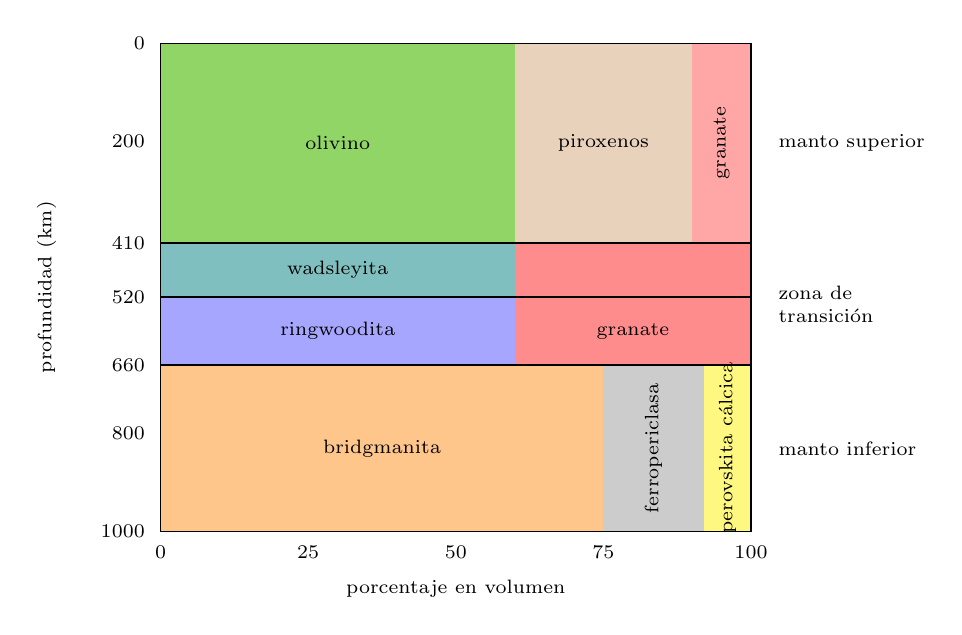
\begin{tikzpicture}[x=0.075mm, y=-0.062mm, font=\scriptsize]
% schematic volume fractions (ledger frost:mantle-transitions, sun:lower-mantle)
\def\W{1000}
% upper mantle 0-410: olivine 60, pyroxenes 30, garnet 10
\fill[green!45!olive!60] (0,0) rectangle (600,410);
\fill[brown!35] (600,0) rectangle (900,410);
\fill[red!35] (900,0) rectangle (1000,410);
% 410-520 wadsleyite 60, garnet 40 ; 520-660 ringwoodite 60, garnet 40
\fill[teal!50] (0,410) rectangle (600,520);
\fill[blue!35] (0,520) rectangle (600,660);
\fill[red!45] (600,410) rectangle (1000,660);
% 660-1000 bridgmanite 75, ferropericlase 17, Ca-perovskite 8
\fill[orange!45] (0,660) rectangle (750,1000);
\fill[gray!40] (750,660) rectangle (920,1000);
\fill[yellow!50] (920,660) rectangle (1000,1000);
\draw (0,0) rectangle (1000,1000);
\foreach \d in {410,520,660} \draw[thick] (0,\d) -- (1000,\d);
\node at (300,205) {olivino};
\node[align=center] at (750,205) {piroxenos};
\node[rotate=90] at (950,205) {granate};
\node at (300,465) {wadsleyita};
\node at (300,590) {ringwoodita};
\node[align=center] at (800,590) {granate};
\node at (375,830) {bridgmanita};
\node[rotate=90, align=center] at (835,830) {ferropericlasa};
\node[rotate=90] at (960,830) {perovskita cálcica};
\foreach \d in {0,200,410,520,660,800,1000} \node[anchor=east] at (-10,\d) {\d};
\node[rotate=90, anchor=south] at (-160,500) {profundidad (km)};
\foreach \p in {0,25,50,75,100} \node[anchor=north] at (\p*10,1010) {\p};
\node[anchor=north] at (500,1080) {porcentaje en volumen};
\node[anchor=west, align=left] at (1030,205) {manto superior};
\node[anchor=west, align=left] at (1030,535) {zona de\\transición};
\node[anchor=west, align=left] at (1030,830) {manto inferior};
\end{tikzpicture}

\par\smallskip{\small Los \omterm{def:b1:rock-forming-minerals:mineral}{minerales} de un \omterm{def:b1:layered-earth:layers}{manto} de peridotita con la profundidad, como fracciones de volumen (esquema: las
fronteras se dibujan nítidas, y las fracciones son valores redondos dentro de los intervalos citados en el texto). La composición no
cambia; los \omterm{def:b1:rock-forming-minerals:mineral}{minerales} sí, hacia \qty{410}{km}, \qty{520}{km} y \qty{660}{km}.}
\end{omfigure}

En la base del \omterm{def:b1:layered-earth:layers}{manto}, la capa llamada D$''$ (D doble prima, nombre conservado de un modelo temprano de la Tierra) tiene un gradiente de
velocidad distinto del resto del \omterm{def:b1:layered-earth:layers}{manto} inferior; el PREM le asigna los \qty{150}{km} más bajos del \omterm{def:b1:layered-earth:layers}{manto}. Es heterogénea
sísmicamente: parches de velocidad muy baja, gradientes empinados, reflectores. Se cree que es una capa límite entre el núcleo
caliente y el \omterm{def:b1:layered-earth:layers}{manto}, y quizá un cementerio de losas antiguas.
% ledger: prem:dpp

\section{El núcleo}

El núcleo es sobre todo hierro. Su densidad, sus velocidades y su capacidad de generar un campo magnético apuntan a un metal,
y el hierro es, con mucho, el elemento más abundante de entre los bastante densos que muestran los meteoritos y el Sol. El níquel,
abundante en los meteoritos de hierro, lo acompaña. Pero el núcleo no es hierro--níquel puro.
\begin{itemize}
  \item El núcleo es un \qtyrange{5}{10}{\percent} menos denso que el hierro puro a la misma presión y temperatura: debe contener
        elementos ligeros, entre los que los candidatos son silicio, azufre, carbono, oxígeno e hidrógeno.
  \item La densidad salta en unos \qty{4.5}{\percent} en la \omterm{def:b1:layered-earth:discontinuity}{frontera del núcleo interno}, demasiado para la solidificación de un
        mismo metal: el \omterm{def:b1:layered-earth:layers}{núcleo interno} también contiene elementos ligeros, pero menos, unos pocos por ciento frente al
        \qtyrange{5}{10}{\percent} del líquido.
\end{itemize}
% ledger: badro:core
La diferencia tiene una consecuencia. A medida que la Tierra se enfría ---su \omterm{def:b1:layered-earth:layers}{manto} unos \qty{100}{\degreeCelsius} por mil millones
de años en la actualidad---, el líquido del núcleo se solidifica sobre el \omterm{def:b1:layered-earth:layers}{núcleo interno}, que crece, y
% ledger: bellini:cooling
la solidificación deja la mayor parte de los elementos ligeros en el líquido. El líquido ligero liberado en la base del \omterm{def:b1:layered-earth:layers}{núcleo
externo} sube, y se cree que esta flotabilidad ayuda a agitar el \omterm{def:b1:layered-earth:layers}{núcleo externo} y a impulsar la dinamo que genera el campo
magnético terrestre.

\section{Capas mecánicas: litosfera y astenosfera}

Las capas de arriba se definen por composición y fase: \omterm{def:b1:layered-earth:layers}{corteza} y \omterm{def:b1:layered-earth:layers}{manto} son rocas distintas, \omterm{def:b1:layered-earth:layers}{núcleo externo} e interno son estados
distintos. La tectónica de placas necesita otra división, por resistencia, que atraviesa la primera.

\begin{definition}[Litosfera, astenosfera, zona de baja velocidad]
\label{def:b1:layered-earth:lithosphere}
La \emph{litosfera}\index{litosfera} es la cáscara rígida exterior de la Tierra, la \omterm{def:b1:layered-earth:layers}{corteza} y el \omterm{def:b1:layered-earth:layers}{manto} más superior, que se
comporta como una capa resistente a lo largo de los tiempos geológicos y está dividida en placas. La
\emph{astenosfera}\index{astenosfera} es la capa más débil del \omterm{def:b1:layered-earth:layers}{manto} superior situada debajo, que se deforma por un flujo lento y
deja que las placas se muevan. La \emph{zona de baja velocidad}\index{zona de baja velocidad} es el intervalo de profundidad
bajo la litosfera en el que las velocidades sísmicas, sobre todo las de las ondas S, son menores que justo encima y debajo.
\end{definition}

La \omterm{def:b1:layered-earth:lithosphere}{litosfera} no es una roca sino un intervalo de temperaturas: la peridotita del \omterm{def:b1:layered-earth:layers}{manto} es resistente donde está fría y se
arrastra donde está caliente, y su base es, aproximadamente, una isoterma. Es delgada bajo las dorsales, donde sube el \omterm{def:b1:layered-earth:layers}{manto}
caliente, tiene unos \qty{140}{km} de espesor bajo el fondo oceánico más antiguo, y \qtyrange{40}{280}{km} bajo los continentes,
más gruesa bajo los cratones antiguos; la parte superior de la \omterm{def:b1:layered-earth:lithosphere}{astenosfera} está a unos \qtyrange{80}{200}{km}. Sísmicamente, la
\omterm{def:b1:layered-earth:lithosphere}{astenosfera} se manifiesta como la \omterm{def:b1:layered-earth:lithosphere}{zona de baja velocidad}, cerca de sus condiciones de fusión: en el PREM la velocidad S disminuye
ligeramente desde el \omterm{def:b1:layered-earth:discontinuity}{Moho} hasta \qty{220}{km}, donde vuelve a subir de golpe. Cómo depende la resistencia de la temperatura, y
por qué, es el tema de \cref{ch:b1:stress-strain-rheology}.

\begin{inthefield}[A seismic station]
\begin{minipage}[t]{0.55\linewidth}\vspace{0pt}
Los tiempos de viaje en los que descansan los modelos de referencia proceden de estaciones permanentes. Un sismómetro de banda
ancha, que registra los movimientos del suelo desde centésimas de segundo hasta horas de periodo, se asienta sobre un pilar de
hormigón apoyado en roca desnuda y aislado del suelo de la cámara, bajo una cubierta que mantiene su temperatura estable: un
cambio de una fracción de grado, una corriente de aire o un camión que pasa aparecerían en el registro. El registrador de datos
marca cada muestra con la hora que proporcionan los satélites, y los registros llegan por flujo a centros de datos que los
comparten abiertamente. Las redes de estas estaciones localizan y datan cada gran terremoto; las llegadas elegidas en sus
registros se invirtieron para obtener las velocidades a cada profundidad.
\end{minipage}\hfill
\begin{minipage}[t]{0.42\linewidth}\vspace{0pt}
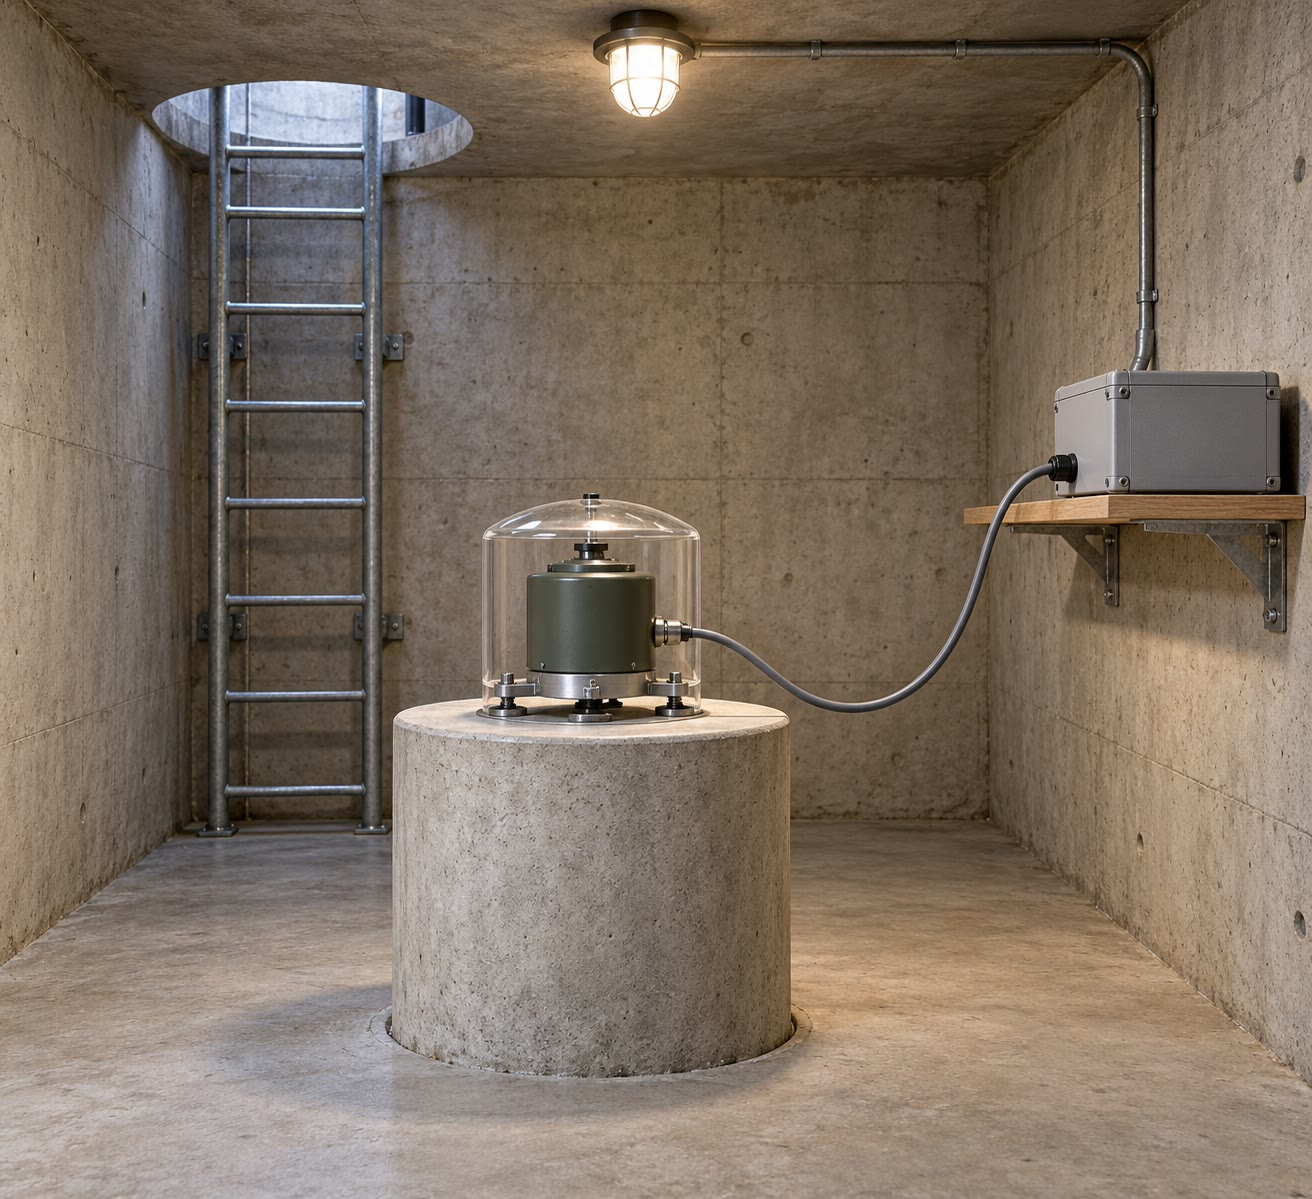
\includegraphics[width=\linewidth]{images/book3/ai/b1-seismometer-vault.jpg}

{\scriptsize Un sismómetro de banda ancha sobre su pilar en una cámara subterránea, con el registrador de datos en la pared
(ilustración generada por IA).}
\end{minipage}
\end{inthefield}

\section{Ejercicios}

\begin{exercise}[$\star$]\label{exo:b1:layered-earth:1}
Con los radios del PREM $R = \qty{6371}{km}$, $r_{\text{CMB}} = \qty{3480}{km}$ y $r_{\text{ICB}} = \qty{1221.5}{km}$,
calcúlense las fracciones del volumen de la Tierra que ocupan el núcleo y el \omterm{def:b1:layered-earth:layers}{núcleo interno}.
% ledger: prem:cmb, prem:icb
\end{exercise}

\begin{exercise}[$\star$]\label{exo:b1:layered-earth:2}
Justo encima de la \omterm{def:b1:layered-earth:discontinuity}{frontera núcleo--manto} el PREM da $v_P = \qty{13.7166}{km.s^{-1}}$, $v_S = \qty{7.26466}{km.s^{-1}}$,
$\rho = \qty{5.56645}{g.cm^{-3}}$; justo debajo, $v_P = \qty{8.06482}{km.s^{-1}}$, $v_S = 0$, $\rho = \qty{9.90349}{g.cm^{-3}}$.
Calcúlense el \omterm{def:b1:layered-earth:seismic-parameter}{parámetro sísmico} y el módulo de compresión a cada lado (en GPa). ¿Qué cambia más a través de la frontera?
% ledger: data:prem, prem:cmb
\end{exercise}

\begin{exercise}[$\star$]\label{exo:b1:layered-earth:3}
Una \omterm{def:b1:layered-earth:layers}{corteza} de \qty{30}{km} de espesor, a \qty{6.2}{km.s^{-1}}, se apoya en un \omterm{def:b1:layered-earth:layers}{manto} a \qty{8.1}{km.s^{-1}}. Calcúlense el
ángulo crítico, la distancia crítica y la \omterm{def:b1:layered-earth:head-wave}{distancia de cruce}.
\end{exercise}

\begin{exercise}[$\star$]\label{exo:b1:layered-earth:4}
La masa del núcleo es \qty{1.94e24}{kg} y su radio \qty{3480}{km}. Calcúlese la gravedad en la \omterm{def:b1:layered-earth:discontinuity}{frontera núcleo--manto} y
compárese con la gravedad en la superficie, \qty{9.82}{m.s^{-2}}. ¿Por qué es mayor?
\end{exercise}

\begin{exercise}[$\star\star$]\label{exo:b1:layered-earth:5}
En un perfil de refracción las primeras llegadas están a \qty{10.0}{s} a \qty{60}{km}, a \qty{33.3}{s} a \qty{200}{km} y a
\qty{45.8}{s} a \qty{300}{km}; la recta que pasa por el primer punto atraviesa el origen. Hállense $v_1$, $v_2$, el tiempo de
intersección y la profundidad de la frontera, y compruébese el resultado con la \omterm{def:b1:layered-earth:head-wave}{distancia de cruce}.
\end{exercise}

\begin{exercise}[$\star\star$]\label{exo:b1:layered-earth:6}
Demuéstrese que una esfera uniforme tiene $I = 0.4\,MR^2$. Calcúlense después la masa y el factor $I/MR^2$ de una Tierra de dos
capas: un núcleo de radio \qty{3480}{km} y densidad \qty{11.0}{g.cm^{-3}} en un \omterm{def:b1:layered-earth:layers}{manto} de densidad \qty{4.45}{g.cm^{-3}}, con
$R = \qty{6371}{km}$. Compárense con \num{5.972e24} kg y $0.3308$.
\end{exercise}

\begin{exercise}[$\star\star$]\label{exo:b1:layered-earth:7}
A \qty{1471}{km} de profundidad el PREM da $v_P = \qty{12.16}{km.s^{-1}}$, $v_S = \qty{6.673}{km.s^{-1}}$, $\rho = \qty{4.86}{g.cm^{-3}}$,
y la gravedad es \qty{9.9}{m.s^{-2}}. Calcúlese el gradiente de densidad que da la ecuación de Adams--Williamson, en
\unit{g.cm^{-3}} por \qty{1000}{km}, y compárese con las densidades del PREM, \num{4.844} a \qty{1471}{km} y \num{5.357} a
\qty{2471}{km}.
% ledger: data:prem
\end{exercise}

\begin{exercise}[$\star\star$]\label{exo:b1:layered-earth:8}
Estímese la presión a \qty{670}{km} de profundidad a partir de una densidad media de \qty{3.57}{g.cm^{-3}} y una gravedad de
\qty{9.9}{m.s^{-2}}. ¿Qué cambio \omterm{def:b1:rock-forming-minerals:mineral}{mineral} se espera allí?
% ledger: frost:mantle-transitions
\end{exercise}

\begin{exercise}[$\star\star$]\label{exo:b1:layered-earth:9}
La densidad media del \omterm{def:b1:layered-earth:layers}{núcleo externo} en el PREM es \qty{10.90}{g.cm^{-3}}; en la \omterm{def:b1:layered-earth:discontinuity}{frontera del núcleo interno} su densidad es
\qty{12.166}{g.cm^{-3}} por encima y \qty{12.764}{g.cm^{-3}} por debajo. (a)~Si el hierro en las mismas condiciones es un
\qtyrange{5}{10}{\percent} más denso que el \omterm{def:b1:layered-earth:layers}{núcleo externo}, ¿qué intervalo de densidades da para el hierro líquido allí?
(b)~Calcúlese el salto de densidad en la \omterm{def:b1:layered-earth:discontinuity}{frontera del núcleo interno} en tanto por ciento, y compárese con el \qty{4.5}{\percent}
de estudios recientes. (c)~¿Qué diría un salto
mayor que el que da la sola congelación sobre los elementos ligeros?
% ledger: badro:core, prem:icb
\end{exercise}

\begin{exercise}[$\star\star\star$]\label{exo:b1:layered-earth:10}
Demuéstrese que el tiempo de la onda reflejada $t_r(x) = \sqrt{x^2 + 4h^2}/v_1$ y el tiempo de la \omterm{def:b1:layered-earth:head-wave}{onda de cabeza} de
\cref{thm:b1:layered-earth:two-layer} son iguales, con pendientes iguales, en $x = 2h\tan i_c$, y que $t_r > t_{\text{cabeza}}$
más allá. Interprétese.
\end{exercise}

\begin{exercise}[$\star\star\star$]\label{exo:b1:layered-earth:11}
Para una Tierra de densidad uniforme $\rho$, demuéstrese que $g(r) = \tfrac43\pi G\rho r$ y
$P(r) = \tfrac23\pi G\rho^2(R^2 - r^2)$. Calcúlese la presión central con $\rho = \qty{5513}{kg.m^{-3}}$ y
$R = \qty{6371}{km}$, y compárese con los \qty{363.85}{GPa} del PREM.
% ledger: earth:density, prem:centre
\end{exercise}

\begin{exercise}[$\star\star\star$]\label{exo:b1:layered-earth:12}
Demuéstrese que si $g/\Phi$ es constante a través de una capa, la ecuación de Adams--Williamson da
$\rho = \rho_0\exp\bigl(g(z - z_0)/\Phi\bigr)$ con la profundidad $z$. Aplíquese al \omterm{def:b1:layered-earth:layers}{núcleo externo}, desde
\qty{2891}{km} ($\rho_0 =
\qty{9.90}{g.cm^{-3}}$) hasta \qty{5149.5}{km}, con los valores medios
$g = \qty{7.9}{m.s^{-2}}$ y $\Phi = \qty{87}{km^2.s^{-2}}$; compárese con los \qty{12.17}{g.cm^{-3}} del PREM en la \omterm{def:b1:layered-earth:discontinuity}{frontera
del núcleo interno}.
% ledger: prem:icb
\end{exercise}

\section{Problema: pesar las cáscaras de la Tierra}

\begin{problem}[{Problema de fin de semana --- volúmenes, masas y momento de inercia de una Tierra de cuatro cáscaras construida
con el PREM, comparados con la masa y el momento de inercia medidos; gravedad y presión en el interior profundo}]
\label{pb:b1:layered-earth:1}
% values: calc/ch09.py; mean densities rounded from figdata prem_profiles (values part)
% ledger: data:prem, prem:constraints, prem:centre, prem:cmb, earth:mass, earth:MoI, const:G
La Tierra se divide en cuatro cáscaras en los radios del PREM, y a cada una se le asigna su densidad media en el PREM,
redondeada:
\begin{center}
\small
\begin{tabular}{lccc}
\hline
capa & desde (km) & hasta (km) & densidad media (\unit{g.cm^{-3}}) \\
\omterm{def:b1:layered-earth:layers}{corteza}, \omterm{def:b1:layered-earth:layers}{manto} superior y zona de transición & 5701 & 6371 & 3.57 \\
\omterm{def:b1:layered-earth:layers}{manto} inferior & 3480 & 5701 & 4.90 \\
\omterm{def:b1:layered-earth:layers}{núcleo externo} & 1221.5 & 3480 & 10.90 \\
\omterm{def:b1:layered-earth:layers}{núcleo interno} & 0 & 1221.5 & 12.89 \\
\hline
\end{tabular}
\end{center}
Úsese $G = \qty{6.674e-11}{m^3.kg^{-1}.s^{-2}}$. La masa medida de la Tierra es \qty{5.972e24}{kg} y su \omterm{def:b1:comparative-planetology:moi}{factor de momento
de inercia} $I/MR^2 = 0.3308$.

\medskip
\noindent\textbf{Parte I --- Volúmenes.}
\begin{enumerate}
  \item Calcúlese el volumen de la Tierra.
  \item Calcúlese el volumen de cada cáscara.
  \item ¿Qué fracción del volumen ocupa cada cáscara? ¿Cuál es la mayor?
  \item ¿Qué fracción del volumen es núcleo?
\end{enumerate}

\noindent\textbf{Parte II --- Masas.}
\begin{enumerate}[resume]
  \item Calcúlese la masa de cada cáscara.
  \item Súmense, y compárese el total con la masa medida.
  \item Dedúzcase la densidad media de la Tierra modelo.
  \item ¿Qué fracción de la masa está en el \omterm{def:b1:layered-earth:layers}{núcleo interno}?
  \item ¿Qué fracción de la masa está en el \omterm{def:b1:layered-earth:layers}{manto} y la \omterm{def:b1:layered-earth:layers}{corteza} juntos?
  \item Compárese la parte del núcleo en el volumen y en la masa, y explíquese.
\end{enumerate}

\noindent\textbf{Parte III --- Momento de inercia.}
\begin{enumerate}[resume]
  \item Muéstrese a partir de \cref{prop:b1:layered-earth:integrals} que una cáscara uniforme entre $r_1$ y $r_2$ tiene
        $I = \tfrac{8\pi}{15}\rho\,(r_2^5 - r_1^5)$.
  \item Calcúlese el momento de inercia de cada cáscara.
  \item ¿Qué cáscara aporta más, y por qué el \omterm{def:b1:layered-earth:layers}{núcleo interno} aporta casi nada?
  \item Súmense y calcúlese $I/MR^2$ para el modelo.
  \item Compárese con $0.3308$ y con el $0.4$ de una esfera uniforme.
  \item Dentro de cada cáscara real la densidad aumenta con la profundidad. ¿Explica eso por qué el factor del modelo es demasiado
        alto? Explíquese.
\end{enumerate}

\noindent\textbf{Parte IV --- Gravedad y presión.}
\begin{enumerate}[resume]
  \item Calcúlese la gravedad en la superficie del modelo.
  \item Calcúlese la gravedad en la \omterm{def:b1:layered-earth:discontinuity}{frontera núcleo--manto}.
  \item Calcúlese la densidad media del \omterm{def:b1:layered-earth:layers}{manto} y la \omterm{def:b1:layered-earth:layers}{corteza} juntos.
  \item La gravedad en el \omterm{def:b1:layered-earth:layers}{manto} se mantiene cerca de \qty{10}{m.s^{-2}}. Estímese la presión en la \omterm{def:b1:layered-earth:discontinuity}{frontera núcleo--manto}, y
        compárese con los \qty{135.75}{GPa} del PREM.
  \item Calcúlese la densidad media del núcleo, y el aumento de presión desde la \omterm{def:b1:layered-earth:discontinuity}{frontera núcleo--manto} hasta el centro en un
        núcleo uniforme, $\tfrac23\pi G\rho_c^2 r_c^2$ (\cref{exo:b1:layered-earth:11} aplicado solo al núcleo).
  \item Súmense ambas para estimar la presión central, y compárese con los \qty{363.85}{GPa} del PREM. ¿Por qué la estimación
        es demasiado baja?
  \item ¿Cuáles de los números del modelo se comprueban con una medida, y cuáles solo con el propio PREM?
  \item ¿Qué fracción de la masa de la Tierra está en el núcleo?
\end{enumerate}
\end{problem}
